\documentclass[11pt]{article}
\usepackage[T1]{fontenc}
\usepackage{lmodern,microtype}
\usepackage[a4paper,margin=27mm]{geometry}
\usepackage{amsmath,amssymb,amsthm,mathtools,booktabs,array}
\usepackage[dvipsnames]{xcolor}
\usepackage{tikz}
\usepackage[colorlinks=true,linkcolor=MidnightBlue,citecolor=MidnightBlue,urlcolor=MidnightBlue]{hyperref}
\usepackage[nameinlink,noabbrev]{cleveref}
\usepackage{fancyhdr}
\pagestyle{fancy}\fancyhf{}
\fancyhead[L]{\small Sub-quorum colorings and boundary matchings}
\fancyhead[R]{\small Working draft}
\fancyfoot[C]{\thepage}
\setlength{\headheight}{14pt}
\newtheorem{theorem}{Theorem}[section]
\newtheorem{lemma}[theorem]{Lemma}
\newtheorem{proposition}[theorem]{Proposition}
\newtheorem{corollary}[theorem]{Corollary}
\theoremstyle{definition}
\newtheorem{definition}[theorem]{Definition}
\newtheorem{question}[theorem]{Question}
\theoremstyle{remark}
\newtheorem{remark}[theorem]{Remark}
\newcommand{\psq}{\psi_{\mathrm{sq}}}
\newcommand{\bii}{\beta_2}
\newcommand{\R}{\mathbb R}
\newcommand{\Om}{\Omega}
\newcommand{\norm}[1]{\left\lVert#1\right\rVert}
\DeclareMathOperator{\diag}{diag}
\title{From hypercubes to grids:\\sub-quorum colorings and structural bounds}
\author{Wenlin Zhang\thanks{Working draft prepared for discussion with Rafik Sahbi.
The author list and contribution statement will be settled jointly.}\\
\small National University of Singapore; The Omega Institute}
\date{27 September 2026}
\begin{document}
\maketitle
\begin{abstract}
We prove that the sub-quorum coloring number of the $n$-dimensional
hypercube is $2^{n-1}$ for every $n\ge2$, resolving Sahbi's Conjecture~6.4.
The proof combines a reduction to selected color representatives with
Huang's signed adjacency matrix. An energy estimate yields an injective
boundary map and, more strongly, a boundary matching covering all selected
edge-free representatives. Starting from this solution, we pursue two
directions: rectangular grids and the structural conditions for equality
between the sub-quorum coloring number and the $2$-independence number.
For grids, exact integer transfer certificates establish Sahbi's proposed
formula at widths $8$, $9$, $10$, and $11$ for every positive length.
For the structural question, we extend the boundary argument to bipartite
graphs with an orthogonal signed adjacency matrix and their Cartesian
products. An exact grafting formula also produces trees of maximum degree
three on which the difference between the two parameters is arbitrarily
large. The hypercube coloring-number equality is formalized in Lean~4;
the grid certificates are checked by two implementations of the transfer.
\end{abstract}

\section{Introduction}

A sub-quorum coloring allows vertices to remain uncolored, while requiring
each colored vertex to have a weak majority of its colored closed
neighborhood in its own color. The maximum number of colors, denoted
$\psq(G)$, therefore depends on both a chosen induced subgraph and a
partition of that subgraph. This parameter was introduced in the study of
quorum colorings by Hedetniemi, Hedetniemi, Laskar, and Mulder~\cite{HHLM}.
Sahbi~\cite{Sahbi} developed its structural and computational theory and
posed the following question for the Boolean cube $Q_n$.

\begin{theorem}[Sahbi's Conjecture 6.4]\label{thm:main}
For every integer $n\ge2$,
\[
 \psq(Q_n)=\bii(Q_n)=2^{n-1}.
\]
Here $\bii(G)$ is the largest cardinality of a vertex set inducing maximum
degree at most one.
\end{theorem}

Sahbi proved the full equality for dimensions $2$ through $6$ and established
$\bii(Q_n)=2^{n-1}$ for every $n\ge2$ using Huang's theorem.
The remaining step was the general upper bound for $\psq$. His reduction to an auxiliary
parameter $\Om$ turns the problem into a boundary comparison: for a set
$T$ of selected representatives and a vertex-disjoint matching $M$, put
$A=T\cup V(M)$ and $B=V(Q_n)\setminus A$. The desired estimate is
$|T|\le |B|$. The elementary edge count gives only
$(n-1)|T|\le n|B|$, leaving a gap.

We close that gap using the signed adjacency operator from Huang's proof
of the Sensitivity Conjecture~\cite{Huang}. If $x$ is supported on $T$, its
image has total squared norm $n\norm{x}^2$, whereas at most
$(n-1)\norm{x}^2$ can lie on $A$. Consequently restriction to $B$ is
injective. The same estimate applies to every subset of $T$ and proves the
Hall inequalities for a matching from $T$ to $B$.

The solved hypercube problem is the starting point for two further
questions. The first concerns rectangular grids: can a boundary argument
prove Sahbi's proposed formula for arbitrary width and length? Straight
two-step paths prevent the square-scalar signing used for cubes. We use
Sahbi's transfer method to establish four additional widths, each for
every positive length. Their complete state-vector certificates give
exact cases against which a uniform boundary inequality can be tested.

The second question is structural: which graphs satisfy $\psq=\bii$?
The hypercube proof supplies a sufficient condition for a class of
regular bipartite graphs and their Cartesian products. In the other
direction, an exact grafting formula gives trees of maximum degree three
with an unbounded additive gap. Together with nonheredity of the equality
class, these results identify both a mechanism for equality and constraints
on a broader characterization.

\section{Partial colorings and the matching reduction}\label{sec:reduction}

All graphs are finite, simple, and undirected. Write $N_G(v)$ for the open
neighborhood and $N_G[v]=N_G(v)\cup\{v\}$ for the closed neighborhood.
A sub-quorum coloring is a surjection $f:S\to\{1,\ldots,k\}$, where
$S\subseteq V(G)$ and $k\ge1$, such that for every $v\in S$,
\begin{equation}\label{eq:quorum}
 2\bigl|\{u\in N_G[v]\cap S:f(u)=f(v)\}\bigr|
 \ge |N_G[v]\cap S|.
\end{equation}
The center is counted once and uncolored neighbors do not enter either
side. The maximum attainable $k$ is $\psq(G)$. For a graph with no vertices we use
the convention $\psq=0$. If $a(v)$ counts same-color neighbors and $d_S(v)$
counts all colored neighbors, \eqref{eq:quorum} is equivalent to
\begin{equation}\label{eq:local}
 d_S(v)\le 1+2a(v).
\end{equation}
In particular a colored vertex with no same-color neighbor has colored
degree at most one.

Every set inducing maximum degree at most one can be colored with one
color per vertex. Hence Sahbi's elementary lower bound is
\begin{equation}\label{eq:lower}
 \bii(G)\le\psq(G).
\end{equation}

\begin{definition}[Sahbi's auxiliary parameter]
A pair $(T,M)$ is feasible if $M$ is a matching, $T\cap V(M)=\varnothing$,
and each $t\in T$ has at most one neighbor in $T\cup V(M)$. Define
\[
 \Om(G)=\max\{|T|+|M|:(T,M)\text{ is feasible}\}.
\]
\end{definition}

\begin{lemma}[Matching reduction]\label[lemma]{lem:reduction}
For every finite graph $G$, $\psq(G)\le\Om(G)$.
\end{lemma}
\begin{proof}
Take any admissible $k$-coloring. For each color class containing an edge,
select one such edge. For each remaining color class, select one vertex.
The selected edges form a matching $M$ and the selected vertices form a
set $T$ disjoint from its endpoints. Each vertex of $T$ has no same-color
neighbor, so \eqref{eq:local} bounds its colored degree by one. Since all
selected vertices are colored, $(T,M)$ is feasible. Exactly one item was
selected for each color, so $k=|T|+|M|\le\Om(G)$.
\end{proof}

This is the reduction of Sahbi's Lemma~5.4, expressed directly for arbitrary
partial colorings. The distinction between classes containing an edge and
edge-free classes avoids a preliminary connectedness normalization.

\section{A boundary injection and a boundary matching}\label{sec:boundary}

A signed adjacency matrix of $G$ is a real symmetric matrix $S$ whose entry
$S_{uv}$ belongs to $\{-1,1\}$ when $uv\in E(G)$ and is zero otherwise.

\begin{theorem}[Boundary matching]\label{thm:boundary}
Suppose $G$ has a signed adjacency matrix satisfying
\begin{equation}\label{eq:square}
 S^2=dI,\qquad d\ge2.
\end{equation}
For every feasible pair $(T,M)$, put $A=T\cup V(M)$ and $B=V(G)\setminus A$.
Then the bipartite graph consisting of the edges between $T$ and $B$ has
a matching saturating $T$. In particular,
\begin{equation}\label{eq:omega-half}
 \Om(G)\le |V(G)|/2.
\end{equation}
\end{theorem}
\begin{proof}
The diagonal entries of \eqref{eq:square} show that $G$ is $d$-regular.
Every $t\in T$ has at most one neighbor in $A$. Every $a\in A$ has at most
$d-1$ neighbors in $T$: if $a\in T$, this follows from $1\le d-1$; if
$a\in V(M)$, its matched partner is a neighbor outside $T$.

Extend $x\in\R^T$ by zero to $V(G)$. For each $a\in A$, Cauchy--Schwarz
gives
\[
 (Sx)_a^2\le |N(a)\cap T|\sum_{t\in N(a)\cap T}x_t^2.
\]
Sum first over $a$ and then over $t$ to obtain
\begin{align}
 \norm{(Sx)|_A}^2
 &\le(d-1)\sum_{t\in T}|N(t)\cap A|x_t^2\notag\\
 &\le(d-1)\norm{x}^2.\label{eq:restricted}
\end{align}
Symmetry and \eqref{eq:square} give $\norm{Sx}^2=d\norm{x}^2$, whence
\begin{equation}\label{eq:boundary-energy}
 \norm{(Sx)|_B}^2\ge\norm{x}^2.
\end{equation}
Thus $x\mapsto(Sx)|_B$ is injective and $|T|\le|B|$.

More precisely, let $U\subseteq T$. Restrict the domain to vectors
supported on $U$. Their boundary images are supported on
$N_B(U)=N_G(U)\cap B$, and \eqref{eq:boundary-energy} still gives
injectivity. Comparing dimensions yields $|U|\le|N_B(U)|$ for every $U$.
Hall's theorem now supplies the asserted matching. Finally,
\[
 2(|T|+|M|)=|A|+|T|\le |A|+|B|=|V(G)|,
\]
which proves \eqref{eq:omega-half}.
\end{proof}

\begin{corollary}\label[corollary]{cor:bipartite}
If $G$ is bipartite and satisfies the hypotheses of
\cref{thm:boundary}, then
\[
 \bii(G)=\psq(G)=\Om(G)=|V(G)|/2.
\]
\end{corollary}
\begin{proof}
Regularity with positive degree implies that the two bipartition classes
have equal cardinality. Either class is independent, so it gives the
lower bound $|V|/2$ in \eqref{eq:lower}. Apply \cref{lem:reduction,thm:boundary}.
\end{proof}

\subsection{The hypercube conjecture}

Huang's signed matrices can be defined recursively by
\[
 S_1=\begin{pmatrix}0&1\\1&0\end{pmatrix},\qquad
 S_{n+1}=\begin{pmatrix}S_n&I\\I&-S_n\end{pmatrix}.
\]
They have exactly the edge support of $Q_n$, are symmetric, and satisfy
$S_n^2=nI$ by direct block multiplication~\cite{Huang}.
For $n\ge2$, \cref{cor:bipartite} proves \cref{thm:main}.
The lower-bound coloring assigns a distinct color to each even-parity
vertex and leaves all odd-parity vertices uncolored.

The same argument proves the boundary-matching strengthening for every
feasible $(T,M)$ in a cube. This supplies a Hall-type conclusion along
Sahbi's proposed boundary route, with feasibility retained explicitly.

\begin{remark}\label[remark]{rem:feasible}
The matching hypothesis on $A\setminus T$ matters. The condition
$|N(t)\cap A|\le1$ alone does not guarantee a matching from $T$ to $B$.
In $Q_2$, take $T$ to be two opposite vertices and let $A$ also contain
one of the remaining vertices. Then $|T|=2$ and $|B|=1$, while every
$t\in T$ has exactly one neighbor in $A$. Such an $A$ cannot be written
as $T\cup V(M)$ with $M$ disjoint from $T$.
\end{remark}

\section{Products and the limits of the signing method}\label{sec:products}

\begin{proposition}[Cartesian products]\label[proposition]{prop:product}
Let $G,H$ be bipartite graphs with signed adjacency matrices $S_G,S_H$
satisfying $S_G^2=d_GI$ and $S_H^2=d_HI$, where $d_G,d_H>0$. Their
Cartesian product has such a matrix with square $(d_G+d_H)I$. Consequently
\[
 \bii(G\mathbin\square H)=\psq(G\mathbin\square H)
 =\Om(G\mathbin\square H)=\frac{|V(G)||V(H)|}{2}.
\]
\end{proposition}
\begin{proof}
Let $J_G$ be diagonal, equal to $1$ on one bipartition class and $-1$ on
the other. Since edges cross the bipartition,
$J_GS_G=-S_GJ_G$. Define
\[
 S=S_G\otimes I+J_G\otimes S_H.
\]
The summands have disjoint supports on the two types of product edges.
Thus $S$ is a symmetric signed adjacency matrix, and its cross terms
cancel on squaring:
\[
 S^2=d_GI+I\otimes d_HI=(d_G+d_H)I.
\]
The product is bipartite and $d_G+d_H\ge2$, so apply \cref{cor:bipartite}.
\end{proof}

For example, a Hadamard matrix $H$ of order $r$ gives a signing
\[
 S=\begin{pmatrix}0&H\\H^{\mathsf T}&0\end{pmatrix}
\]
of $K_{r,r}$ with $S^2=rI$. Order four is supplied by
\[
 H=\begin{pmatrix}
 1&1&1&1\\1&-1&1&-1\\1&1&-1&-1\\1&-1&-1&1
 \end{pmatrix}.
\]
Products involving $K_{4,4}$ and cubes therefore give examples beyond the
cube family. The exact value for complete bipartite graphs already follows
from Sahbi's complete-multipartite result; here the signing also gives
the boundary matching and a product construction.

\begin{proposition}[A local obstruction]\label[proposition]{prop:unique}
If two distinct vertices have exactly one common neighbor, then $G$
admits no signed adjacency matrix with square a scalar multiple of $I$.
\end{proposition}
\begin{proof}
If $z$ is the unique common neighbor of $u,v$, then
$(S^2)_{uv}=S_{uz}S_{zv}\in\{-1,1\}$, whereas every off-diagonal entry
of a scalar matrix vanishes.
\end{proof}

In a rectangular grid with a side of length at least three, two vertices
two steps apart along a straight line have exactly one common neighbor.
Thus the cube signing cannot be transferred unchanged to these grids.
The obstruction concerns this matrix method, not the proposed grid equality.

\section{An unbounded gap on connected trees}\label{sec:trees}

Sahbi's survey of earlier work~\cite{Sahbi} records exact sub-quorum
numbers for some caterpillar families. Here we study the difference
between the two parameters and exhibit a connected family on which it
grows without bound.

Let $D$ be the double star with centers $u,v$, leaves $a,b$ adjacent to
$u$, and leaves $c,d$ adjacent to $v$. Its four leaves form a
$2$-independent set. If both centers are selected, no leaf can be selected;
if exactly one center is selected, at most one of its own leaves and the
two opposite leaves can be selected. Hence $\bii(D)=4$.
Coloring the centers together and all four leaves separately gives five
sub-quorum colors. Six distinct colors violate the condition at a center,
so $\psq(D)=5$.

\begin{figure}[ht]
\centering
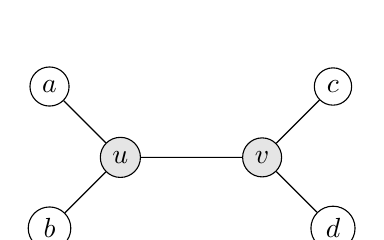
\begin{tikzpicture}[scale=.9,every node/.style={circle,draw,inner sep=2.6pt}]
\node[fill=gray!20] (u) at (0,0) {$u$};
\node[fill=gray!20] (v) at (2,0) {$v$};
\node (a) at (-1,1) {$a$};\node (b) at (-1,-1) {$b$};
\node (c) at (3,1) {$c$};\node (d) at (3,-1) {$d$};
\draw (u)--(v) (u)--(a) (u)--(b) (v)--(c) (v)--(d);
\end{tikzpicture}
\caption{The double star $D$: the centers share one color and each leaf
has its own color. Thus $\psq(D)=5>4=\bii(D)$.}
\label{fig:double}
\end{figure}

This example can be amplified while preserving connectedness.

\begin{theorem}\label{thm:treegap}
For $k\ge1$, form $H_k$ from $k$ disjoint copies $D_i$ of $D$ by adding a
new vertex $h$ and edges $ha_i$, one to a designated leaf in each copy.
Then $H_k$ is a tree on $6k+1$ vertices and
\[
 \bii(H_k)=4k+1,\qquad \psq(H_k)=5k.
\]
In particular $\psq(H_k)-\bii(H_k)=k-1$ is unbounded.
\end{theorem}
\begin{proof}
Restrict a $2$-independent set to each $D_i$: it has at most four vertices
there, and at most one additional vertex is $h$. This gives $4k+1$ as
an upper bound. It is attained by selecting $h$ and, in each copy, the set
$\{u_i,b_i,c_i,d_i\}$. The selected edges are just $u_ib_i$.

Leaving $h$ uncolored and using the five-color construction in every
copy gives $5k$ colors. To prove the upper bound, restrict any sub-quorum
coloring to each $D_i$. This restriction is still admissible. Only $a_i$
loses a neighbor, and after deletion it has degree at most one, which
always satisfies the sub-quorum condition. Let $c_i$ be the number of
colors represented in $D_i$; then $c_i\le5$.

If $h$ is uncolored, or its color occurs in some $D_i$, the total number
of colors is at most $\sum_i c_i\le5k$. Otherwise its color is new, so
the only possible violation of the bound would require every $c_i=5$.
An admissible five-coloring of $D_i$ must color all six vertices: a support
of five vertices with five colors would be $2$-independent, contradicting
$\bii(D_i)=4$. It therefore has exactly one two-vertex color class.
Each degree-three center must have a same-color neighbor, so this class
must be $\{u_i,v_i\}$. All leaves have distinct colors. In $H_k$, the
vertex $a_i$ then has two colored neighbors, $u_i$ and $h$, both of a
different color from its own. This violates \eqref{eq:local}. Thus some
$c_i\le4$, and even with the new hub color the total is at most $5k$.
\end{proof}

\begin{theorem}[An exact grafting formula]\label{thm:grafting}
Let $F$ be a nonempty graph on vertices $h_1,\ldots,h_k$. Form $R(F)$
by adding disjoint copies $D_i$ of $D$ and the edges $h_ia_i$. Then
\[
 \bii(R(F))=4k+\bii(F),\qquad \psq(R(F))=5k.
\]
\end{theorem}
\begin{proof}
A $2$-independent set contains at most four vertices of each $D_i$ and
at most $\bii(F)$ vertices of $F$. To attain this bound, take an optimal
set in $F$ and $\{u_i,b_i,c_i,d_i\}$ in each copy. None of the vertices
$a_i$ is selected, so the attachment edges introduce no new constraint.

Leaving $F$ uncolored gives $5k$ sub-quorum colors. For the reverse bound,
restrict an arbitrary admissible coloring to each $D_i$. As in the proof
above, this is admissible; let $c_i\le5$ count its colors. Let $r$ be the
number of colors occurring exclusively in $F$, and choose one vertex
$h_i$ representing each such color. The chosen indices are distinct.
If $c_i=5$, both centers in $D_i$ have one common color and each leaf has
its own color. Then $a_i$ sees two colored neighbors, $u_i$ and $h_i$,
neither of its own color, a contradiction. Each chosen index therefore
has $c_i\le4$. The total number of colors is at most
\[
 \sum_i c_i+r\le5k-r+r=5k.
\]
This argument permits arbitrary edges within $F$.
\end{proof}

\begin{corollary}\label[corollary]{cor:subcubic}
There are trees of maximum degree three with arbitrarily large difference
$\psq-\bii$. Specifically, $R(P_k)$ has $7k$ vertices and
\[
 \bii(R(P_k))=4k+\left\lceil\frac{2k}{3}\right\rceil,
 \qquad \psq(R(P_k))=5k,
\]
so the difference is $\lfloor k/3\rfloor$.
\end{corollary}
\begin{proof}
Every three consecutive vertices of a path contain at most two vertices
of a $2$-independent set. Selecting two out of every three attains
$\bii(P_k)=\lceil2k/3\rceil$. Apply \cref{thm:grafting}.
All vertices of $R(P_k)$ have degree at most three, and the centers have
degree exactly three.
\end{proof}

Within this grafted family, $\psq(R(F))=\bii(R(F))$ holds exactly when
$\bii(F)=k$, equivalently when $F$ itself has maximum degree at most one.

\begin{corollary}\label[corollary]{cor:nonhereditary}
The class of graphs satisfying $\psq=\bii$ is not hereditary.
\end{corollary}
\begin{proof}
The graph $D$ is an induced subgraph of the $3\times4$ rectangular grid:
place its centers at $(2,2),(2,3)$ and its leaves at
$(1,2),(2,1),(2,4),(3,3)$. The full grid satisfies
$\psq=\bii=7$ by Sahbi's width-three formula, while $D$ does not.
\end{proof}

In particular the complete equality class has no characterization solely
by forbidden induced subgraphs. This leaves open characterizations using
global conditions, or within restricted classes of host graphs.

\section{Grid strips beyond width seven}\label{sec:grid}

Write $G_{m,n}=P_m\square P_n$ and set
\begin{equation}\label{eq:gridformula}
 F(m,n)=\max\left\{
 \left\lceil\frac m2\right\rceil\left\lceil\frac{2n}3\right\rceil
 +\left\lfloor\frac m2\right\rfloor\left\lfloor\frac n3\right\rfloor,
 \left\lceil\frac n2\right\rceil\left\lceil\frac{2m}3\right\rceil
 +\left\lfloor\frac n2\right\rfloor\left\lfloor\frac m3\right\rfloor
 \right\}.
\end{equation}
Sahbi's Proposition~5.2 gives $\bii(G_{m,n})\ge F(m,n)$. In odd rows,
select columns not divisible by three; in even rows, select columns
divisible by three. There are no selected vertical edges, and every
selected vertex has at most one selected horizontal neighbor. Transposing
the construction gives the other term of \eqref{eq:gridformula}.

\begin{theorem}[Computer-assisted strip extension]\label{thm:strips}
For $m\in\{8,9,10,11\}$ and every integer $n\ge1$,
\[
 \bii(G_{m,n})=\psq(G_{m,n})=\Om(G_{m,n})=F(m,n).
\]
\end{theorem}

We prove the upper bound using the same max-plus propagation principle as
Sahbi's Theorem~5.5, with an independently implemented frontier encoding.
The finite objects, their interpretation, and the induction from the
certificates are given below.

\subsection{Frontier states and exact transfer}

Process the grid in consecutive layers of $m$ vertices, within each layer
from left to right. A frontier contains one digit for each position. A
vertex is called occupied when it belongs to $T\cup V(M)$.

\begin{center}
\begin{tabular}{cl}
\toprule
Digit & Meaning\\\midrule
0 & Unoccupied vertex\\
1 & Vertex in $T$ with no occupied processed neighbor\\
2 & Vertex in $T$ with one occupied processed neighbor\\
3 & Matching endpoint with partner already processed\\
4 & Matching endpoint awaiting its partner in the next layer\\
5 & Matching endpoint awaiting its partner immediately to the right\\
\bottomrule
\end{tabular}
\end{center}

At a new position, the already processed neighbors are the vertex above
and the vertex to the left. The available choices are: leave the position
unoccupied; place a vertex of $T$; close a pending matching edge; or begin
a matching edge to the right or to the next layer. A pending edge must
close when its partner is processed. Two simultaneous requests cannot
share an endpoint. A new occupied vertex is forbidden next to a frontier
vertex of type~2; type~1 changes to type~2 when it gains an occupied
neighbor. A new vertex of $T$ can have at most one occupied past neighbor.
An edge may not point right from the last position of a layer.

Give weight two to a $T$ vertex, weight one to a matching endpoint, and
weight zero to an unoccupied vertex. The transfer retains the maximum
weight among paths reaching the same state. Let $V_n(s)$ be this maximum
after $n$ complete layers, with value $-\infty$ for an unreachable state.
Initially only the all-zero state is reachable, with weight zero.

\begin{lemma}\label[lemma]{lem:transfer}
The transfer computes the optimum over all partial feasible configurations
with the specified frontier. The largest entry of $V_n$ with no pending
matching edge is $2\Om(G_{m,n})$.
\end{lemma}
\begin{proof}
Given a feasible $(T,M)$, orient each matching edge toward its later
endpoint in the processing order. This determines the local choices and
pending requests. At every vertex of $T$, the degree constraint permits
at most one occupied neighbor, so all updates are legal. Thus every
feasible pair has a transfer path.

Conversely, an accepted path defines disjoint $T$ vertices and matching
endpoints. Requests close each matching edge exactly once and prevent
two edges from sharing an endpoint. The updates count every occupied
neighbor of a $T$ vertex when that neighbor is processed and reject any
second one. Vertices forgotten by the frontier have no unprocessed
neighbors, so no condition is lost. A terminal state leaves no matching
edge open, and its weight is exactly $2(|T|+|M|)$. Maximizing proves the
claim.
\end{proof}

\subsection{Finite certificates and all-length induction}

The layer transfer $\Phi_m$ is independent of $n$ and satisfies
$\Phi_m(V+c)=\Phi_m(V)+c$. Thus an equality of complete state vectors
\begin{equation}\label{eq:period}
 V_{a+p}=V_a+\delta
\end{equation}
implies $V_{n+p}=V_n+\delta$ for every $n\ge a$. In particular,
\begin{equation}\label{eq:omega-period}
 \Om(G_{m,n+p})=\Om(G_{m,n})+\delta/2\qquad(n\ge a).
\end{equation}

\begin{center}
\begin{tabular}{rrrrr}
\toprule
Width $m$ & Start $a$ & Period $p$ & Increment $\delta$ & Reachable states\\
\midrule
8 & 9 & 2 & 16 & 40,855\\
9 & 15 & 3 & 28 & 148,196\\
10 & 12 & 2 & 20 & 537,561\\
11 & 16 & 3 & 34 & 1,949,930\\
\bottomrule
\end{tabular}
\end{center}

For each row, the supplied vectors verify \eqref{eq:period} entry by
entry, including identical reachable support. Two implementations compute
both vectors from the initial state. The finite initial values
$1\le n<a+p$ agree with $F(m,n)$.

For completeness, the target formula has the same recurrence in the
required ranges. For even widths eight and ten,
\[
 F(8,n)=\begin{cases}4n&n\text{ even},\\4n+2&n\text{ odd},\end{cases}
 \qquad
 F(10,n)=\begin{cases}5n&n\text{ even},\\5n+2&n\text{ odd}.\end{cases}
\]
For odd widths, write $A_m(n)$ and $B_m(n)$ for the first and second terms
of \eqref{eq:gridformula}. At width nine,
\[
 A_9(n)\ge\frac{14n}{3},\qquad
 B_9(n)\le\frac{9n}{2}+\frac32.
\]
Hence $A_9(n)>B_9(n)$ for $n\ge15$, and $A_9(n+3)=A_9(n)+14$.
At width eleven,
\[
 A_{11}(n)\ge\frac{17n}{3},\qquad
 B_{11}(n)\le\frac{11n}{2}+\frac52.
\]
Thus $A_{11}(n)>B_{11}(n)$ for $n\ge16$, and
$A_{11}(n+3)=A_{11}(n)+17$. These identities, the checked initial values,
and \eqref{eq:omega-period} prove $\Om(G_{m,n})=F(m,n)$ for all lengths.
The construction preceding \cref{thm:strips} and \cref{lem:reduction}
complete its proof.

\section{Verification and reproducibility}\label{sec:verification}

The hypercube equality is formalized in Lean~4 as
\begin{center}
\small\ttfamily
subQuorumChromaticNumber\_hypercube.
\end{center}
The formal definitions preserve the partial support, surjectivity, the
closed-neighborhood convention, and the attained finite maximum. The
proof uses the pinned Mathlib module \texttt{Archive.Sensitivity}, proves
the restricted energy estimate, and obtains the cardinality comparison
through finite-dimensional injectivity. The public source is available at
\begin{center}\small
\url{https://github.com/the-omega-institute/trureturing}
\end{center}
under \path{D5/S3/Combinatorics/Graph/HypercubeSubQuorum.lean}.
The pinned commit is
\begin{center}\small\ttfamily
a53350d0255768f5c26c8b36bf34d47eeb00296f.
\end{center}
The recorded axioms are \texttt{propext}, \texttt{Classical.choice}, and
\texttt{Quot.sound}. The source has SHA256
\begin{center}\scriptsize\ttfamily
7a70d793639d4aabb0b8e44a5871357e474acb0ce2c5f74356241f72767a4a95.
\end{center}

The reproducibility repository is
\begin{center}\small
\url{https://github.com/the-omega-institute/subquorum-colorings}.
\end{center}
It contains the grid transfer programs,
integer state vectors, finite readouts, and verification scripts.
The first C++ implementation constructs vectors and detects translations;
the second enumerates candidate local labels separately and recomputes the
certificate endpoints. Both use exact integer arithmetic. A separate
exhaustive enumeration of matchings and sets $T$ checks small grids.
Constructive lower bounds are checked directly against the finite optima.

For the tree examples, an additional dynamic program is compared with
direct partial-color enumeration on all labelled trees with two through five
vertices and with the six-vertex graph enumeration. It also checks the
family in \cref{thm:treegap} for $1\le k\le30$. These computations support
the direct proofs; they are not needed to infer the arbitrary-$k$ theorem.
The tree recurrence is recorded in \cref{app:tree}.

The grafting formula is additionally checked over all labelled base trees
with two through five vertices, and the subcubic family $R(P_k)$ for
$1\le k\le30$. The general grafting theorem follows from its direct proof.

The Lean theorem proves $\psq(Q_n)=2^{n-1}$ in \cref{thm:main}; it does not
define $\bii$. The $\bii$ identity also follows from the written proof above.
The boundary-matching strengthening,
product theorem, tree family, and grid-strip extension are established by
the arguments and computations in this draft; they have not yet been
formalized in Lean. The two transfer programs share the mathematical
state specification, so their agreement checks implementations rather
than replacing the soundness and completeness proof.

\paragraph{AI-assisted preparation.}
AI tools assisted mathematical exploration, program development,
cross-checking, and preparation of this draft. The formal-verification
scope is specified above. A joint contribution statement will accompany
the version agreed by the collaborators.

\section{Further questions}

The solution of the hypercube conjecture gives a concrete starting point
for the grid and structural questions. Its boundary injection produces
a covering matching. The next task is to understand how much of this
mechanism can survive when the cube's signed-matrix identity is unavailable.

\begin{question}
Can the width-specific transfer certificates be replaced by a boundary
inequality proving $\Om(G_{m,n})\le F(m,n)$ for arbitrary $m,n$?
\end{question}

An upper bound for $\Om$ would prove the proposed grid equality. The strip
certificates provide exact extremal data for separating interior and
boundary contributions and testing candidate inequalities across widths.
A failure of the stronger $\Om$ bound would distinguish the matching
reduction from the original coloring problem.

\begin{question}
Which global structural conditions imply $\psq(G)=\bii(G)$?
\end{question}

The signed boundary theorem supplies a sufficient condition, while
\cref{thm:grafting,cor:subcubic,cor:nonhereditary} constrain possible
characterizations: an unbounded gap already occurs on subcubic trees,
and the full equality class is not hereditary. The exact tree recurrence
provides a setting for identifying additional sufficient conditions and
testing them against explicit obstructions. These two directions extend
the study from a solved family to broader geometric and structural classes.

\appendix
\section{An exact recurrence on trees}\label{app:tree}

For a forest, any color class can be split into its connected components
without changing any same-color adjacency. This preserves all local
constraints and weakly increases the number of colors. We may therefore
assume that color classes induce connected subtrees.

Choose occupation variables $x_v\in\{0,1\}$ and, for each edge, a variable
$y_{uv}\in\{0,1\}$ indicating that its endpoints are colored alike.
Require $y_{uv}\le x_u,x_v$. Since the underlying graph is acyclic, the
components on the occupied vertices joined by selected $y$-edges form a
coloring, with no extra
same-color adjacencies. Its number of colors is
\[
 \sum_v x_v-\sum_{uv\in E}y_{uv}.
\]
For each occupied vertex, the precise local condition is
\begin{equation}\label{eq:tree-local}
 \sum_{u\sim v}x_u\le1+2\sum_{u\sim v}y_{uv}.
\end{equation}
Thus maximizing the displayed objective under these binary constraints
computes $\psq$ exactly on a forest.

Root a tree. Let $P_v(x,p,q)$ be the maximum contribution of the subtree
at $v$, where $x$ is its occupation, $p$ is its parent's occupation, and
$q\le\min(x,p)$ specifies the parent edge. Charge that edge at its child
endpoint. If $w$ runs over the children, the recurrence is
\begin{equation}\label{eq:tree-dp}
 P_v(x,p,q)=x-q+
 \max\left\{\sum_wP_w(x_w,x,q_w):
 \begin{array}{l}
 q_w\le\min(x,x_w),\\
 x=0\ \text{or}\ p+\sum_wx_w\le1+2(q+\sum_wq_w)
 \end{array}\right\}.
\end{equation}
At the root, maximize $P_r(x,0,0)$ over $x\in\{0,1\}$. The all-uncolored
choice has value zero; every nonempty tree has a positive feasible value.
The recurrence follows by splitting the objective and the local condition
at the root of each subtree. Children interact only through their total
occupied and same-color counts, so these totals can be accumulated by a
finite convolution.

For $\bii$, omit the $q$ variables and the edge penalties, and replace the
occupied-vertex condition by $p+\sum_wx_w\le1$. This gives a second exact
recurrence on the same tree. The implementation and comparison checks are
included as \texttt{tree\_parameters.py}.

\begin{thebibliography}{9}
\bibitem{HHLM}
S.~M. Hedetniemi, S.~T. Hedetniemi, R. Laskar, and H.~M. Mulder,
Quorum colorings of graphs,
\emph{AKCE International Journal of Graphs and Combinatorics}
\textbf{10} (2013), 97--109.
\href{https://doi.org/10.1080/09728600.2013.12088727}{doi:10.1080/09728600.2013.12088727}.

\bibitem{Huang}
H. Huang, Induced subgraphs of hypercubes and a proof of the Sensitivity
Conjecture, \emph{Annals of Mathematics} \textbf{190} (2019), 949--955.
\href{https://doi.org/10.4007/annals.2019.190.3.6}{doi:10.4007/annals.2019.190.3.6}.

\bibitem{Sahbi}
R. Sahbi, Sub-quorum colorings of graphs,
\href{https://arxiv.org/abs/2609.25128v1}{arXiv:2609.25128v1} (2026).
\end{thebibliography}
\end{document}
